\chapter{Results}
\label{chap:results}
The following chapter presents the results produced by the analysis method described in chapter \ref{chap:methods} for two different associated and trigger \pt intervals:

The first interval investigated is $\SI{1}{GeV/c} < \ptassoc < \SI{2}{GeV/c} < \pttrig < \SI{4}{GeV/c}$ which was chosen because it is well documented with published results \cite{Abelev2012}. Since this analysis uses a new correction method and different track cuts\footnote{So-called \emph{hybrid} track cuts were used in \cite{Abelev2012}} in comparison to former publications, it was crucial to verify the reproduction of former results. However, the high upper end of the \pttrig interval contradicts the intention of analyzing the softest interactions in hard events and will likely introduce a correlation between the threshold and the trigger particle. Hence, the second interval was chosen to be $\SI{0.5}{GeV/c} < \ptassoc < \SI{1}{GeV/c} < \pttrig < \SI{2}{GeV/c}$ which fulfills the above requirements.\\

This chapter is divided into two parts. The first part deals with the extraction of the double-ridge structure while not requiring a high \pt particle in the event. The results are compared to published results where available in order to demonstrate the correct working of the average-correction method and the here used golden track cuts.\\

The second part of this chapter presents novel findings for events passing the additionally required \ptthresh criteria. Only the second interval is considered here due to the above discussed reasons.

\section[Without high \pt threshold]{Without high \ptbold  threshold}
\label{sec:no-thresh}

The associated yield per trigger particle for the \ptassoc and \pttrig intervals of $ 1 < \ptassoc < \SI{2}{GeV/c} < 2$ and $ 2 < \pttrig < \SI{4}{GeV/c}$ are computed for the $0-20\%$, $20-40\%$, $40-60\%$ and $60-100\%$ multiplicity classes as described in chapter \ref{sec:total_yield}. The yielded outcome for each class is depicted in fig. \ref{fig:Y_no_thresh}. All event classes exhibit the anticipated jet peak on the \gls{near-side} and a ridge like structure on the \gls{away-side} including the jet recoil. A long range \deta structure is clearly recognizable in the two dimension representation for the most central collisions (top left). This effect, however, diminishes with decreasing multiplicity, which can best be observed in the \dphi projection excluding the jet peak region ($|\deta| < 0.8;  \quad \pi /3 < \dphi < 2 \pi /3$); the long-range excess on the nearside decreases in absolute value as well as in comparison to the \gls{away-side} ridge.
\begin{figure}
  \centering
  \begin{subfigure}[b]{0.5\textwidth}
    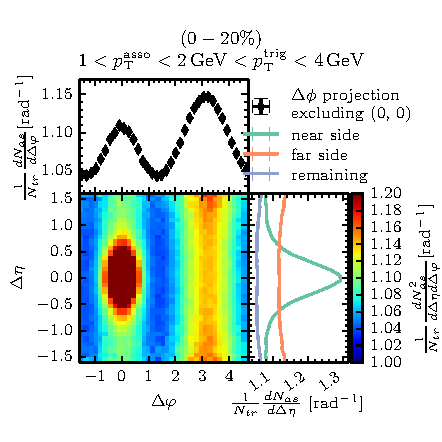
\includegraphics[]{figures/12_24_class0.pdf}
  \end{subfigure}%
  \begin{subfigure}[b]{0.5\textwidth}
    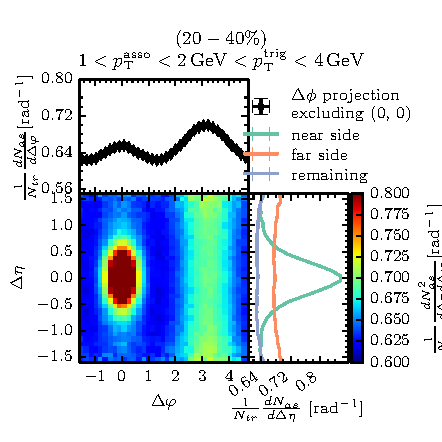
\includegraphics[]{figures/12_24_class1.pdf}
  \end{subfigure}
  \begin{subfigure}[b]{0.5\textwidth}
    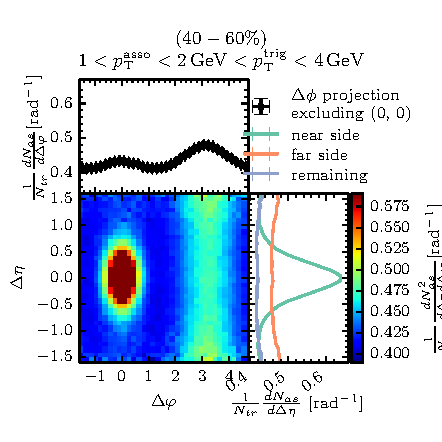
\includegraphics[]{figures/12_24_class2.pdf}
  \end{subfigure}%
  \begin{subfigure}[b]{0.5\textwidth}
    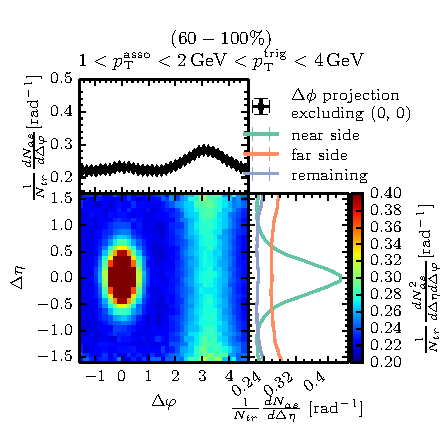
\includegraphics[]{figures/12_24_class3.pdf}
  \end{subfigure}
  \caption[Total associated yield per trigger particle for all four multiplicity classes and the \ptassoc (\pttrig) interval of $1-\SI{2}{GeV/c}$ ($2-\SI{4}{GeV/c}$) and no threshold.]{Total associated yield per trigger particle for all four multiplicity classes and the \ptassoc (\pttrig) interval of $1-\SI{2}{GeV/c}$ ($2-\SI{4}{GeV/c}$). The \dphi projection excludes the jet peak area ($|\deta| < 0.8;  \quad \pi /3 < \dphi < 2 \pi /3$). The long range \deta structure is decreasing in comparison to the \gls{away-side} structure with decreasing multiplicity.}
  \label{fig:Y_no_thresh}
\end{figure}

The multiplicity dependence was further investigated by performing the subtraction method discussed in sec. \ref{sec:subtraction} and fitting the \dphi projection (excluding the peak region ($|\deta| < 0.8;  \quad \pi /3 < \dphi < 2 \pi /3$) to eq. (\ref{eq:double_cosin_fit}). Results are displayed in fig. \ref{fig:comparison_to_pub} (left) along with a comparison to the results published in \cite{Abelev2012} for the same \ptassoc and \pttrig intervals (right). The analysis in the published letter deployed so-called \emph{hybrid} track cuts and corrected with the pair-efficiency method discussed in sec. \ref{sec:single-track-corr}. Furthermore, the expectations from performing this subtraction method on MC reconstructed data (cf. sec. \ref{sec:subtraction}) are displayed in the projection plots as well, underlining that the observed double ridge structure was not anticipated from the MC-simulations. The double cosine fit function (eq. (\ref{eq:double_cosin_fit})) was found to be superior to a single cosine ($a_3 = 0$) fit yielding $\chi ^2 / NDF = 1.29$ compared to $\chi^2 / NDF = 11.75$.

The ridge yield of the here presented method is compatible with the published results, however, the baseline for the yield extraction is found to be  $\sim 5\%$ larger. This can be attributed to an error made in the published results\footnote{The decision was made to not update the public results since it was minor compared to the error of the extracted yields and $v_3$ while $v_2$ is not sensible to $\alpha_{corr}$.}  when applying the finite bin correction to the background normalization as described in sec. \ref{sec:background_distribution}; the inverse of the correction $\alpha_{corr}$ was erroneously applied to the background rendering $B(\deta \approx 0, \dphi \approx 0)$ slightly larger than unity instead of smaller. Exact values of the bin width used in this correction are not available to the author but are expected to be $\sim 5\%$.

\begin{figure}
  \centering
  \begin{subfigure}[b]{0.5\textwidth}
    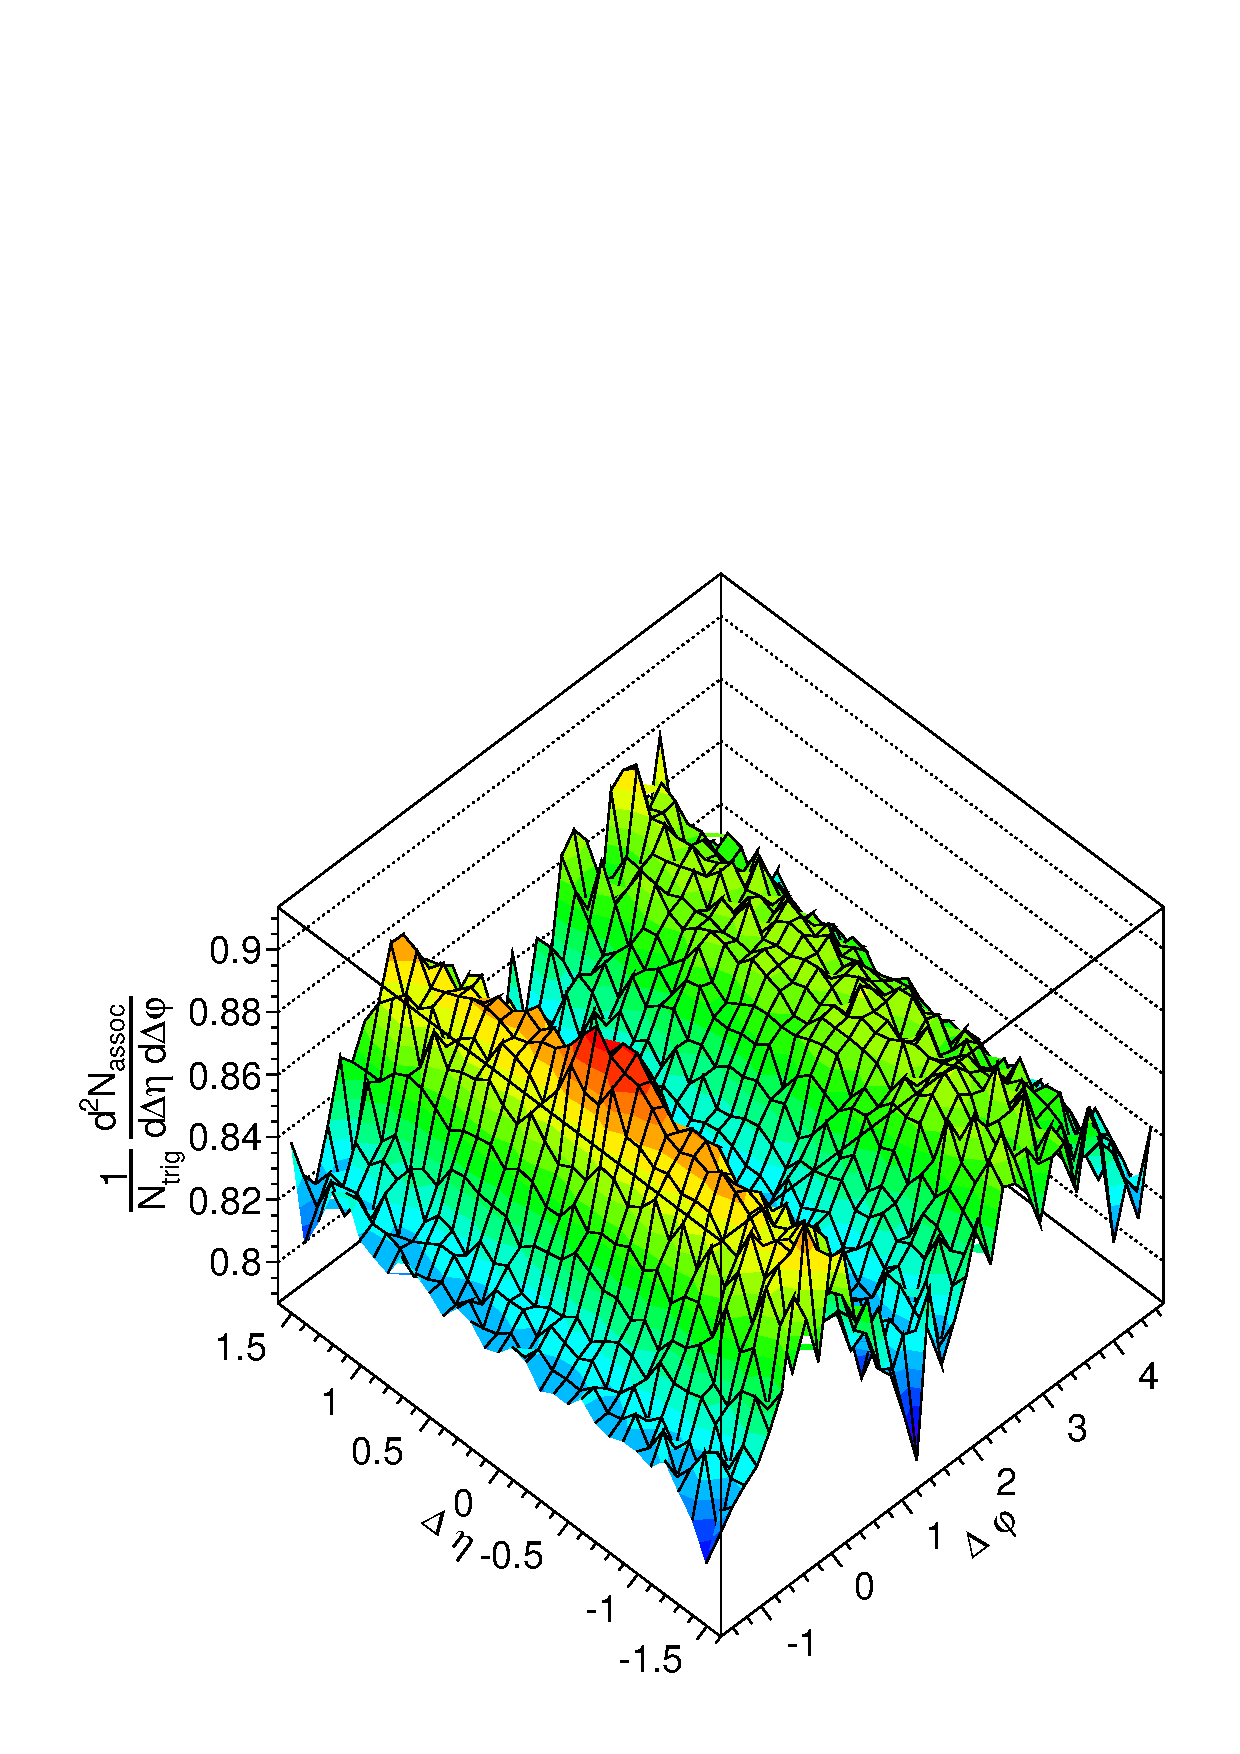
\includegraphics[width=\textwidth]{figures/subtraction_12_24_nothresh.pdf}
  \end{subfigure}%
  \begin{subfigure}[b]{0.5\textwidth}
    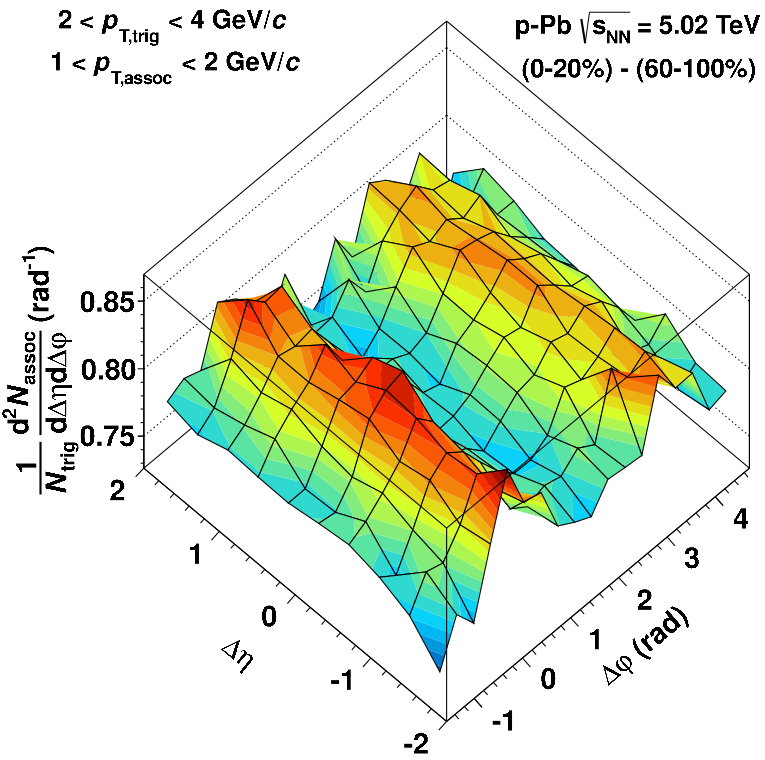
\includegraphics[width=\textwidth]{figures/figures_ALICE_paper/subtraction_plot.png}
  \end{subfigure}
  \begin{subfigure}[b]{0.5\textwidth}
    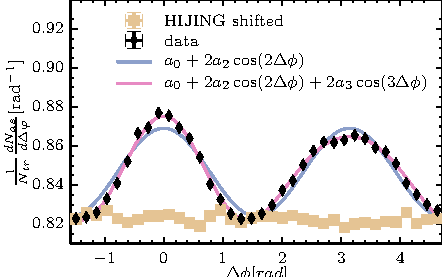
\includegraphics[width=\textwidth]{figures/subtraction_px_12_24_nothresh.pdf}
  \end{subfigure}%
  \begin{subfigure}[b]{0.5\textwidth}
    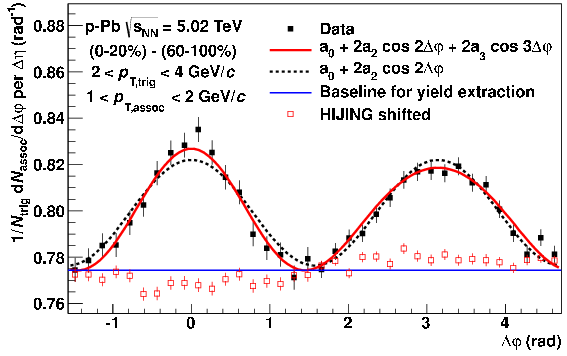
\includegraphics[width=\textwidth]{figures/figures_ALICE_paper/projection_to_phi_without_peak.png}
  \end{subfigure}
  \caption[Subtraction of low multiplicity $Y(\deta, \dphi )$ from that computed for the high multiplicity class in the \ptassoc (\pttrig) interval of $1-\SI{2}{GeV/c}$ ($2-\SI{4}{GeV/c}$) and no threshold.]{Subtraction of low multiplicity $Y(\deta, \dphi )$ from that computed for the high multiplicity class in the \ptassoc (\pttrig) interval of $1-\SI{2}{GeV/c}$ ($2-\SI{4}{GeV/c}$). Left hand side: Results obtained with the methods described in chapter \ref{chap:methods} for measured data. Right hand side: Results published in \cite{Abelev2012} for the same \ptassoc and \pttrig intervals but corrected with the pair-efficiency method. The top right plot presents the \deta projection for the \gls{near-side}, \gls{away-side} and remaining region analog to the \deta projection in the left hand plot. Bottom right (\dphi projection) and the \dphi projection in the left hand plot exclude the jet peak region ($|\dphi| < \pi /3$, $0.8 < |\deta| < 1.6$). The method presented in sec.~\ref{chap:methods}  reproduced the published results apart from an offset explained in the text.}
  \label{fig:comparison_to_pub}
\end{figure}

The same analysis was repeated with the $\SI{0.5}{GeV/c} < \ptassoc < \SI{1}{GeV/c} < \pttrig < \SI{2}{GeV/c}$ interval and is summarized in fig.~\ref{fig:no_thresh_summary_0512}. The results from this interval are phenomenologically very similar to the first described interval. Again, a di-jet like structure was dominantly present for all four multiplicity classes while the most central one showed additional enhancement in the near-side long-range region. The subtraction between the highest and lowest multiplicity class is depicted in fig.~\ref{fig:subtractions_high_pt}(top left) exhibiting the double ridge. The \deta projection in this plot also shows a small remainder of a jet-peak on the near side suggesting that the di-jet contributions are in fact not identical in the high and low multiplicity class.

\begin{figure}
  \centering
  \begin{subfigure}[b]{0.5\textwidth}
    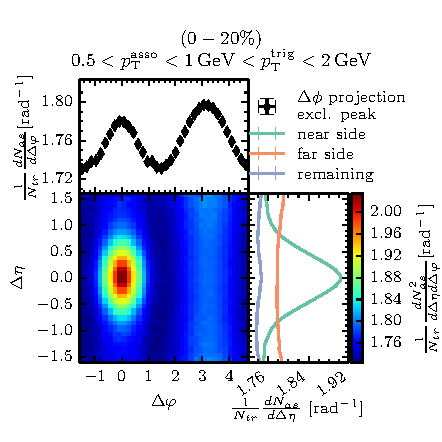
\includegraphics[]{figures/051_12_class0.pdf}
  \end{subfigure}%
  \begin{subfigure}[b]{0.5\textwidth}
    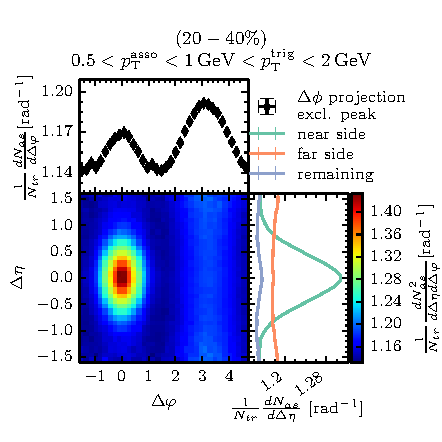
\includegraphics[]{figures/051_12_class1.pdf}
  \end{subfigure}
  \begin{subfigure}[b]{0.5\textwidth}
    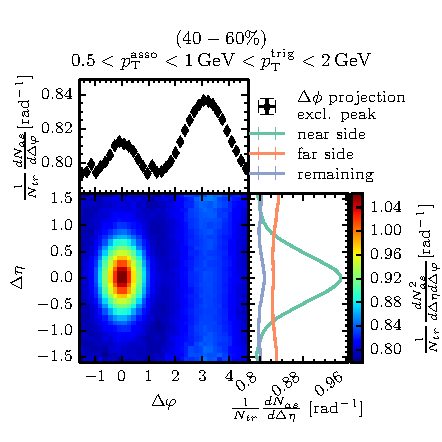
\includegraphics[]{figures/051_12_class2.pdf}
  \end{subfigure}%
  \begin{subfigure}[b]{0.5\textwidth}
    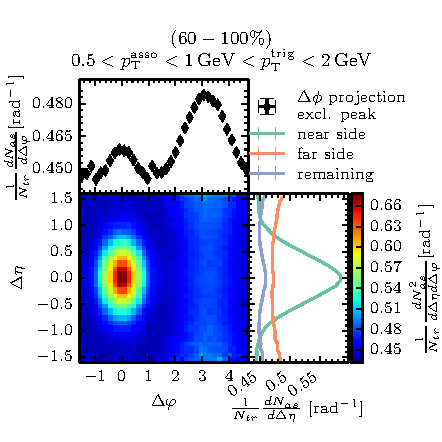
\includegraphics[]{figures/051_12_class3.pdf}
  \end{subfigure}
  \caption[Total associated yield per trigger particle for all four multiplicity classes and the \ptassoc (\pttrig) interval of $1-\SI{2}{GeV/c}$ ($2-\SI{4}{GeV/c}$) and with threshold required.]{Equivalent to fig.~\ref{fig:Y_no_thresh} but for the interval of $\SI{0.5}{GeV/c} < \ptassoc < \SI{1}{GeV/c} < \pttrig < \SI{2}{GeV/c}$. Again, a clear di-jet like structure is seen in all four multiplicity classes while only the highest one $(0-20\%)$ also exhibits an enhancement in the long-range regions of the near-side.}
  \label{fig:no_thresh_summary_0512}
\end{figure}



\section{With high \pt threshold}
\label{sec:with-thres}

The following presents the results with the additional high \pt threshold in the event selection as described in sec. \ref{sec:enrich_hard}.

Fig.~\ref{fig:y_px_thresh} (top) displays the evolution of \Y with increasing \ptthresh projected onto \dphi for each event class. The peak region was excluded in the projections and the \ptassoc and \pttrig intervals were set to $0.5 - \SI{1}{GeV/c}$ and $1-\SI{2}{GeV/c}$. In order to highlight the relative changes in each event class the cases with a threshold $\ptthresh > \SI{0.0}{GeV/c}$ were divided by the results obtained when not requiring a high \pt threshold particle in the event selection criteria (fig. \ref{fig:y_px_thresh} (bottom)). All multiplicity classes exhibited an increase in the number of uncorrelated associated particles per trigger particle (seen as an increase of the baseline), peripheral events were found to have the largest relative gain  in this regard. However, while the uncorrelated contributions were ordered by multiplicity in the projection shown on top, the order was not preserved in the bottom plots: the smallest increase of uncorrelated particles was observed for the $20-40\%$ event class. Regarding changes in the number of correlated particles all but the most central collisions displayed an increase of the away side yield. Furthermore, the most peripheral event class displayed a marginal increase on the near side yield (excluding the peak region).
\begin{figure}
  \centering
  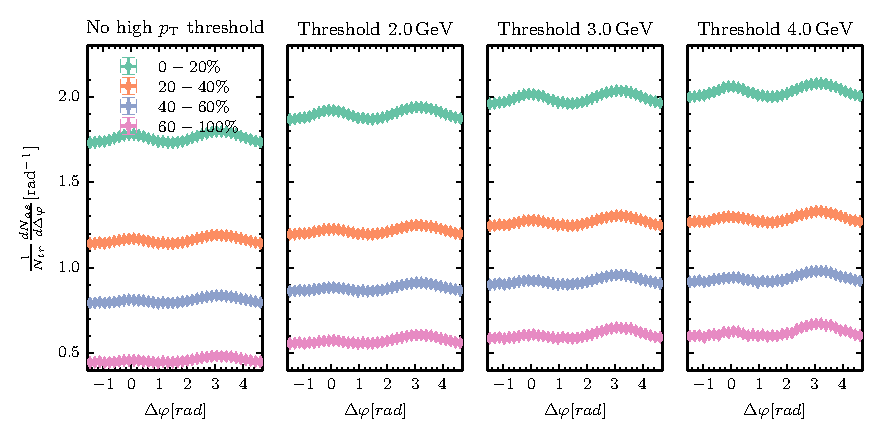
\includegraphics[]{figures/y_px_evolution_with_threshold.pdf}
  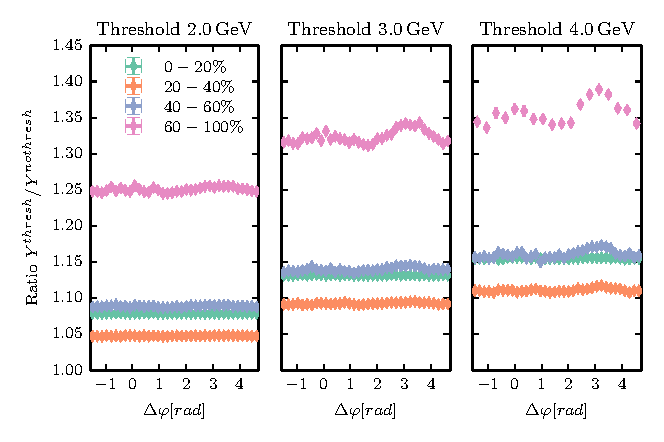
\includegraphics[]{figures/y_px_evolution_with_threshold_div_by_thresh0.pdf}
  \caption[Effect of requiring a high \pt particle in the event selection as projections onto \dphi]{Effect of requiring a high \pt particle in the event selection. Top: Total associated yield per trigger particle as a projection onto \dphi excluding the peak region for several values of \ptthresh . Bottom: The cases with a enforced threshold were divided by the $\ptthresh = \SI{0.0}{GeV/c}$ case to highlight relative changes in each event class. The threshold increased the baseline in all cases. The greatest change in baseline as well as shape was observed for the most peripheral event class. Only statistical uncertainties are shown.}
  \label{fig:y_px_thresh}
\end{figure}

Results for the subtraction method described in sec. \ref{sec:subtraction} in combination with the high \pt threshold requirement are shown in fig. \ref{fig:subtractions_high_pt}. The top left plot represents the no threshold case for comparison. As previously, the peak area was excluded for the \dphi projection to be able to better investigate the long range near side ridge. The results obtained by applying the subtraction method to reconstructed data are shown in light brown in the \dphi projection plots. It was observed that the measured away side yield approached the uncorrelated baseline for increasing values of \ptthresh while the long range contributions to the \gls{near-side} ridge remained largely unchanged. The peak region of the \gls{near-side} peak exhibited the emergence of a dip with increasing threshold as displayed in the \deta projections. 

The change of the \gls{away-side} ridge yield (marked as gray area) can be attributed to the decrease in that area expected from the MC reconstructed data (cf. sec. \ref{sec:subtraction}). This observation was quantified by integrating the difference of the measured and MC reconstructed data over the interval  $\pi / 2 < \dphi < 3\pi/2$. The \gls{near-side} ridge yield was further investigated by separating it into the jet peak area ($|\deta| < 0.8$) and the remaining long range contribution as depicted in fig. \ref{fig:near_side_ridge_yield}. These two areas were integrated over the interval of $-2\pi /2 < \dphi < \pi /2$. The results of these three yield extractions (away-side, near-side and peak region) are shown in fig. \ref{fig:ridge_yield_evo} along with the systematic uncertainties from the MC closure tests described in sec.~\ref{sec:subtraction}. No \ptthresh dependence was found for any of these quantities outside of the margin of uncertainties.


\begin{figure}
  \centering
  \begin{subfigure}[b]{0.5\textwidth}
    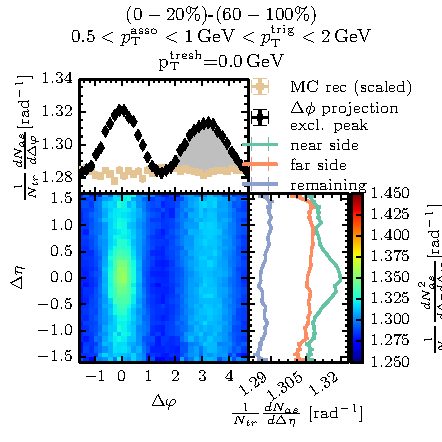
\includegraphics[]{figures/05_12_sub_thresh_00.pdf}
  \end{subfigure}%
  \begin{subfigure}[b]{0.5\textwidth}
    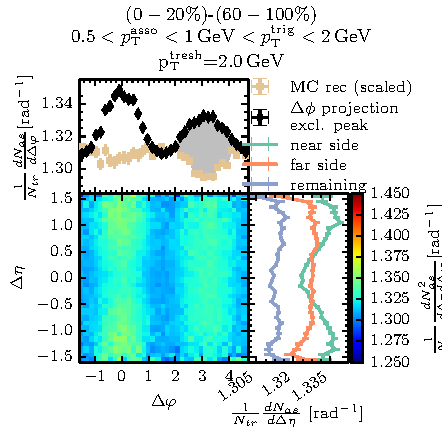
\includegraphics[]{figures/05_12_sub_thresh_20.pdf}
  \end{subfigure}
  \begin{subfigure}[b]{0.5\textwidth}
    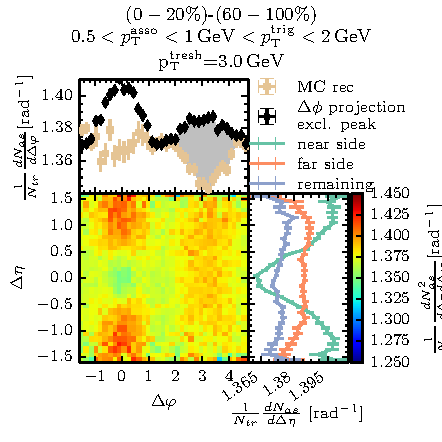
\includegraphics[]{figures/05_12_sub_thresh_30.pdf}
  \end{subfigure}%
  \begin{subfigure}[b]{0.5\textwidth}
    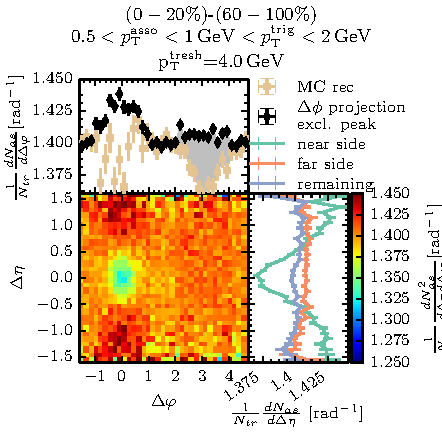
\includegraphics[]{figures/05_12_sub_thresh_40.pdf}
  \end{subfigure}
  \caption[Results for subtracting $60-100\%$ from $(0-20\%)$ for various thresholds.]{Results for subtracting $60-100\%$ from $(0-20\%)$. The results yielded by applying the analysis method onto MC reconstructed data is shown in the \dphi projection in light brown. The area used for the extraction of the far side yield is marked gray. With increasing threshold a dip appears in the near side ridge while the away side ridge appears to vanish. The evolution of the away side yield is depicted in fig. \ref{fig:ridge_yield_evo} }
  \label{fig:subtractions_high_pt}
\end{figure}

\begin{figure}
  \centering
  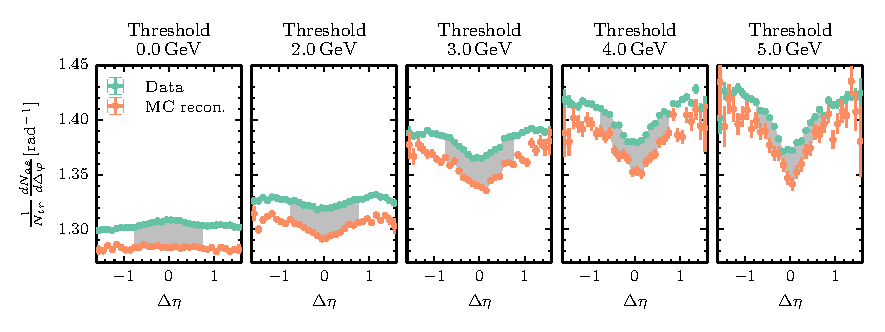
\includegraphics[]{figures/nearside_peak_yield.pdf}
  \caption[Near-side ridge as seen in the \deta projection with MC reconstructed data for various threshold.]{Near-side ridge as seen in the \deta projection. The near side peak was extracted for the region marked grey, the long-range near-side yield was extracted from the region $0.8 < |\deta| < \SI{1.8}{rad}$.}
  \label{fig:near_side_ridge_yield}
\end{figure}

\begin{figure}
  \centering
  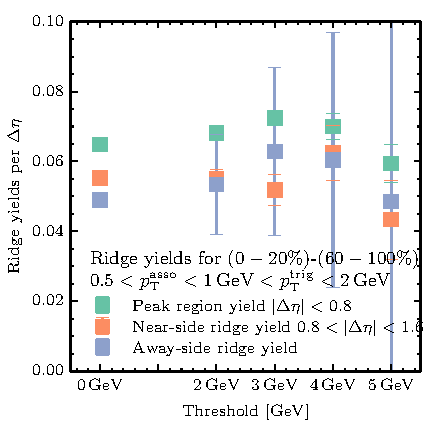
\includegraphics[]{figures/yield_evolution.pdf}
  \caption[Evolution of the ridge yields with increasing threshold.]{Evolution of the ridge yields with increasing threshold. The yields were extracted as described in sec. \ref{sec:yield_extraction} and include the systematic uncertainty introduced by the non-closure at increasing thresholds.}
  \label{fig:ridge_yield_evo}
\end{figure}



%%% Local Variables: 
%%% mode: latex
%%% TeX-master: "main"
%%% End: 